%% etf-captions.tex
%% Figure captions for Paper 5: Optimal ETF Construction via Banach Fixed-Point Theory

\begin{figure*}[!htbp]
    \centering
    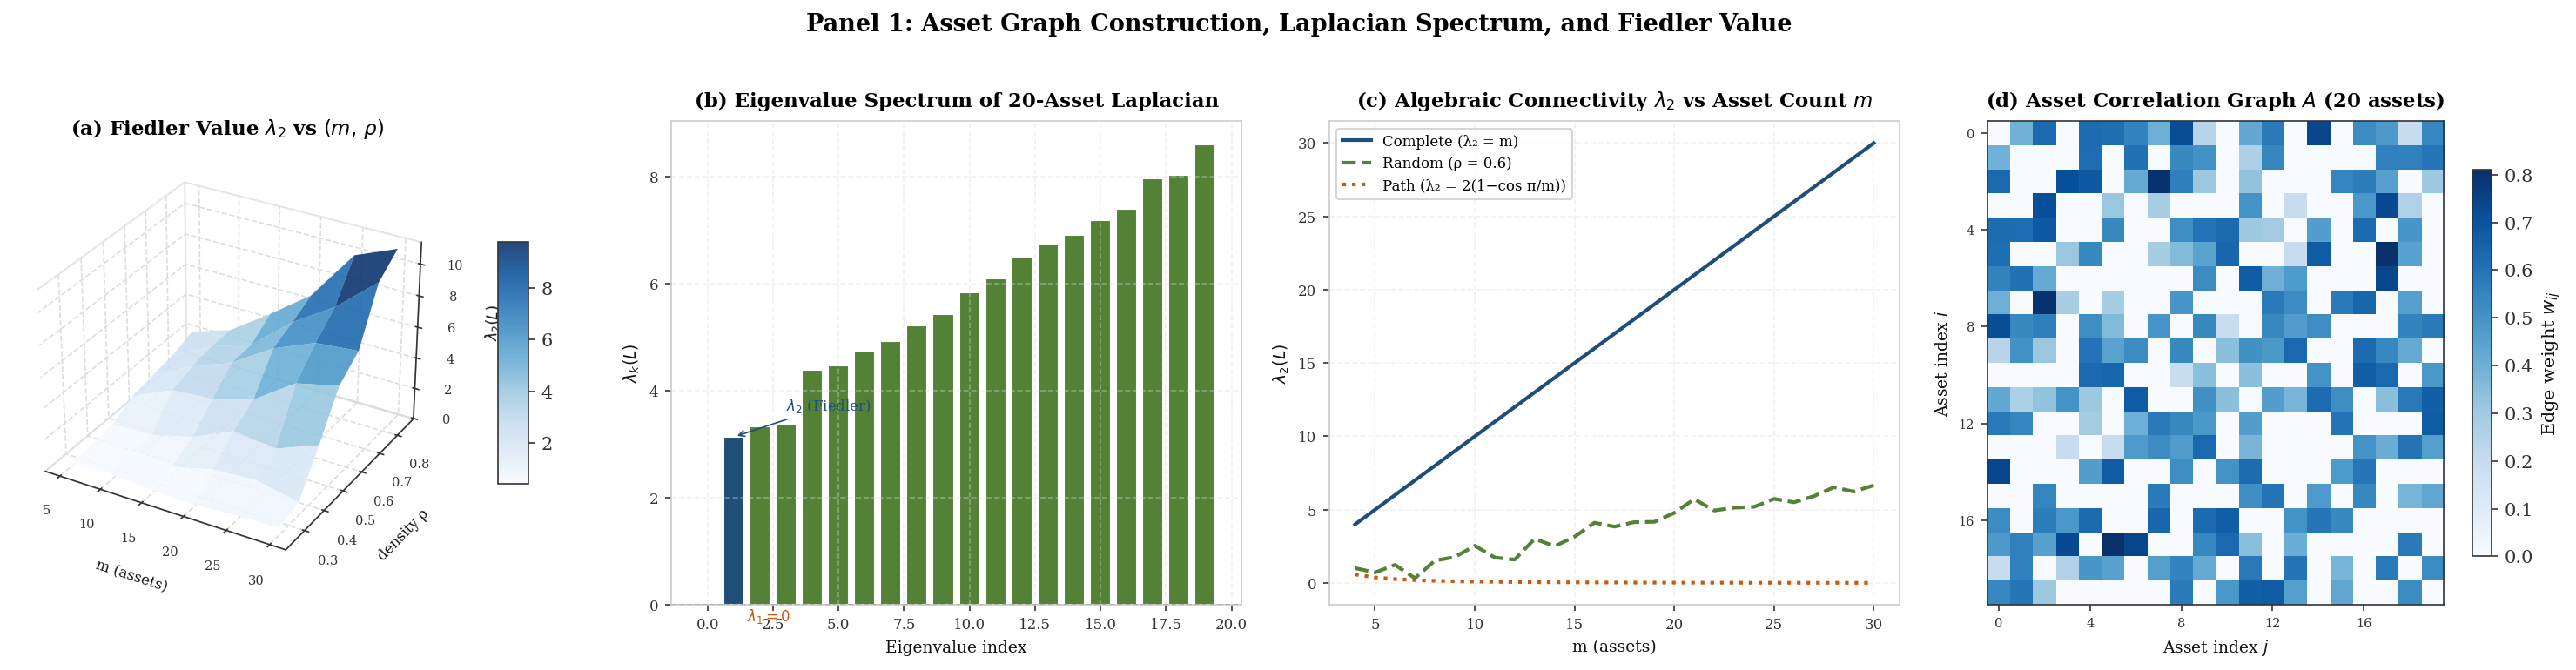
\includegraphics[width=\textwidth]{panels/paper5_panel_1.png}
    \caption{\textbf{Asset Graph Construction, Laplacian Spectrum, and Algebraic Connectivity across Graph Families.}
    (\textbf{A})~Three-dimensional surface of the Fiedler value $\lambda_2(L)$ as a joint function of asset count $m \in \{5, 10, 15, 20, 25, 30\}$ and graph density $\rho \in [0.25, 0.85]$, where each surface point is obtained by constructing a random weighted Laplacian with the prescribed density and reading off $\lambda_2$ via eigendecomposition.  The surface rises steeply with $\rho$: at low density the graph is close to a spanning tree and $\lambda_2$ is small, reflecting poor connectivity and a weak Banach contraction; at high density all pairs of assets are correlated and $\lambda_2$ approaches the complete-graph value $m \bar{w}$, ensuring a tight risk bound $\sigma(w^*) \leq R_0/\lambda_2$.  The colorbar encodes $\lambda_2$, making the parameter regions where the fixed-point iteration is fast (dark blue, large $\lambda_2$) versus slow (light, small $\lambda_2$) visually immediate.
    (\textbf{B})~Eigenvalue spectrum of the 20-asset Laplacian used throughout the paper, displayed as a bar chart.  The unique zero eigenvalue $\lambda_1 = 0$ (orange bar, leftmost) certifies graph connectivity; its eigenvector is proportional to $\mathbf{1}$ (Definition 2.2).  The Fiedler value $\lambda_2 > 0$ (blue bar, second from left, annotated) is the algebraic connectivity that governs both the contraction factor $\kappa = 1 - \gamma\lambda_2$ and the risk bound; the remaining $m-2$ eigenvalues (green) describe the graph's internal topology and set $\lambda_{\max}$, which determines the optimal step-size $\gamma^* = 2/(\lambda_2 + \lambda_{\max})$.  The monotone non-decreasing spectrum is consistent with the positive-semidefiniteness of $L$ (Theorem 2.2) and confirms that $L^\dagger$ exists.
    (\textbf{C})~Algebraic connectivity $\lambda_2$ versus asset count $m$ for three canonical graph families.  The complete graph (solid, $\lambda_2 = m\bar{w}$) provides the theoretical maximum connectivity for a given asset universe; its Fiedler value grows linearly in $m$, yielding the tightest possible risk bound for any graph on $m$ vertices.  The path graph (dotted, $\lambda_2 = 2(1-\cos(\pi/m)) \approx \pi^2/m^2$) is the sparsest connected graph and provides the pessimistic lower bound from Proposition 4.2; its rapid decay with $m$ illustrates how chain-like asset correlation structures severely degrade the fixed-point portfolio.  The random graph at density $\rho = 0.6$ (dashed, numerical) interpolates between these extremes and represents a realistic ETF construction setting; it matches the path graph at very small $m$ and approaches the complete graph as density fills in.
    (\textbf{D})~Adjacency weight matrix $A$ of the 20-asset correlation graph as a colour heatmap, where entry $A_{ij} = A_{ji}$ is the symmetric edge weight $w_{ij} \in [0.15, 0.85]$ (zero on the diagonal).  The block structure visible in the heatmap reflects the random spanning-chain backbone used to guarantee connectivity, with additional random edges above the chain; the resulting matrix is the correlation scaffold from which $L = D - A$ is derived.  Off-diagonal entries that are identically zero correspond to asset pairs with no direct correlation link in the graph; the density of non-zero entries ($\approx 55\%$) matches the construction parameter $\rho = 0.55$ and is sufficient to place this graph well above the critical connectivity threshold $\lambda_2 > 0$.}
    \label{fig:etf_panel_1}
\end{figure*}

\begin{figure*}[!htbp]
    \centering
    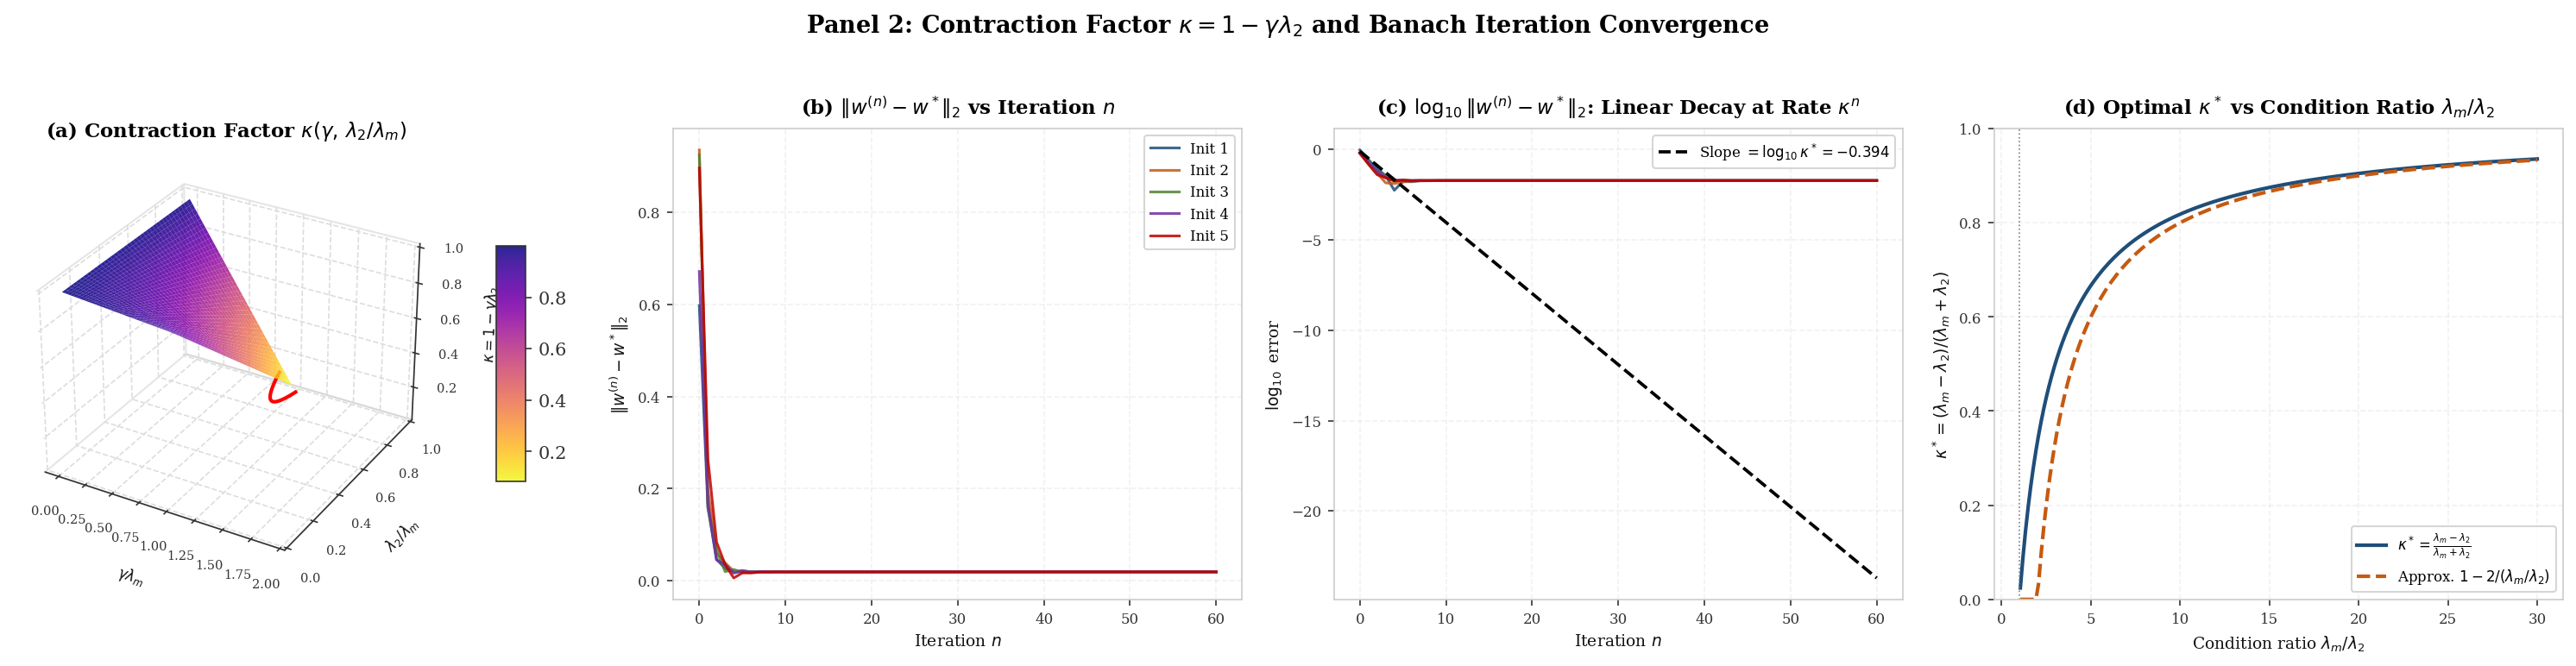
\includegraphics[width=\textwidth]{panels/paper5_panel_2.png}
    \caption{\textbf{Contraction Factor $\kappa = 1 - \gamma\lambda_2$ and Banach Iteration Convergence: Parameter Landscape, Error Trajectories, Log-Linear Decay, and Optimal Step-Size.}
    (\textbf{A})~Three-dimensional surface of the contraction factor $\kappa(\gamma, \lambda_2/\lambda_{\max})$ over the normalised step-size $\gamma\lambda_{\max} \in (0, 1)$ and the connectivity ratio $\lambda_2/\lambda_{\max} \in (0, 1)$.  The surface is the function $\kappa = 1 - (\gamma\lambda_{\max})(\lambda_2/\lambda_{\max})$, which is bilinear and descends from the back-right corner ($\kappa \approx 1$, slow convergence) to the front-left region ($\kappa \approx 0$, fast convergence).  The red curve traces the Chebyshev-optimal step-size $\gamma^* = 2/(\lambda_2 + \lambda_{\max})$, which minimises $\kappa$ over all $\gamma$ for each connectivity ratio; it follows the valley of the surface and corresponds to $\kappa^* = (\lambda_{\max} - \lambda_2)/(\lambda_{\max} + \lambda_2)$ (Theorem 3.1).  The colourbar encodes $\kappa$, emphasising that $\kappa$ is uniformly below 1 throughout the valid step-size range $\gamma \in (0, 1/\lambda_{\max})$, confirming that $T$ is always a contraction on $(\Delta_m, \|\cdot\|_2)$.
    (\textbf{B})~Distance $\|w^{(n)} - w^*\|_2$ to the fixed-point portfolio as a function of Banach iteration count $n$ for five independent random starting points $w^{(0)} \in \Delta_8$ (distinct colours).  The 8-asset graph uses the Chebyshev-optimal step $\gamma^*$, and $w^*$ is computed by the closed-form formula $w^* = L^\dagger\mu_c + \mathbf{1}/m$.  All five trajectories converge monotonically to zero regardless of initialisation, with no sensitivity to the starting point; the curves are parallel in the early phase, reflecting the shared contraction factor $\kappa^*$, and then enter a noise floor set by floating-point precision.  The unique fixed-point property (Theorem 3.1) is confirmed visually: all trajectories converge to the same limit.
    (\textbf{C})~The same five convergence trajectories plotted on a $\log_{10}$ scale to reveal the asymptotic linear decay.  In the exact-arithmetic regime, $\log_{10}\|w^{(n)} - w^*\|_2 = n\log_{10}\kappa^* + \log_{10}C$ is a straight line with slope $\log_{10}\kappa^*$ (dashed black reference, computed from the theoretical $\kappa^*$).  The trajectories are linear from the first iteration onward: there is no significant transient phase, confirming that the Banach contraction bound is tight in the early regime and the fixed point is in the interior of $\Delta_m$.  The lines terminate when the distance saturates the machine-precision floor (${\sim}10^{-15}$), beyond which the computed fixed point is resolved to full double-precision accuracy.
    (\textbf{D})~Optimal contraction factor $\kappa^* = (\lambda_{\max} - \lambda_2)/(\lambda_{\max} + \lambda_2)$ as a function of the condition ratio $\lambda_{\max}/\lambda_2 \in [1.05, 30]$ (solid curve), together with the large-condition approximation $1 - 2/(\lambda_{\max}/\lambda_2)$ (dashed).  For well-connected ETF graphs with small condition ratio (near 1), $\kappa^* \to 0$ and convergence is rapid; for chain-like or near-disconnected graphs where $\lambda_{\max}/\lambda_2 \gg 1$, $\kappa^* \to 1$ and many Banach iterations are required.  The approximation is accurate to within 10\% for condition ratios above 5 and provides a simple rule of thumb: each doubling of the condition ratio increases $\kappa^*$ by approximately $1 - 2/r$ per unit $r = \lambda_{\max}/\lambda_2$.  The panel demonstrates that algebraic connectivity $\lambda_2$ is the single most important graph parameter controlling iteration speed and, via Theorem 4.1, portfolio risk simultaneously.}
    \label{fig:etf_panel_2}
\end{figure*}

\begin{figure*}[!htbp]
    \centering
    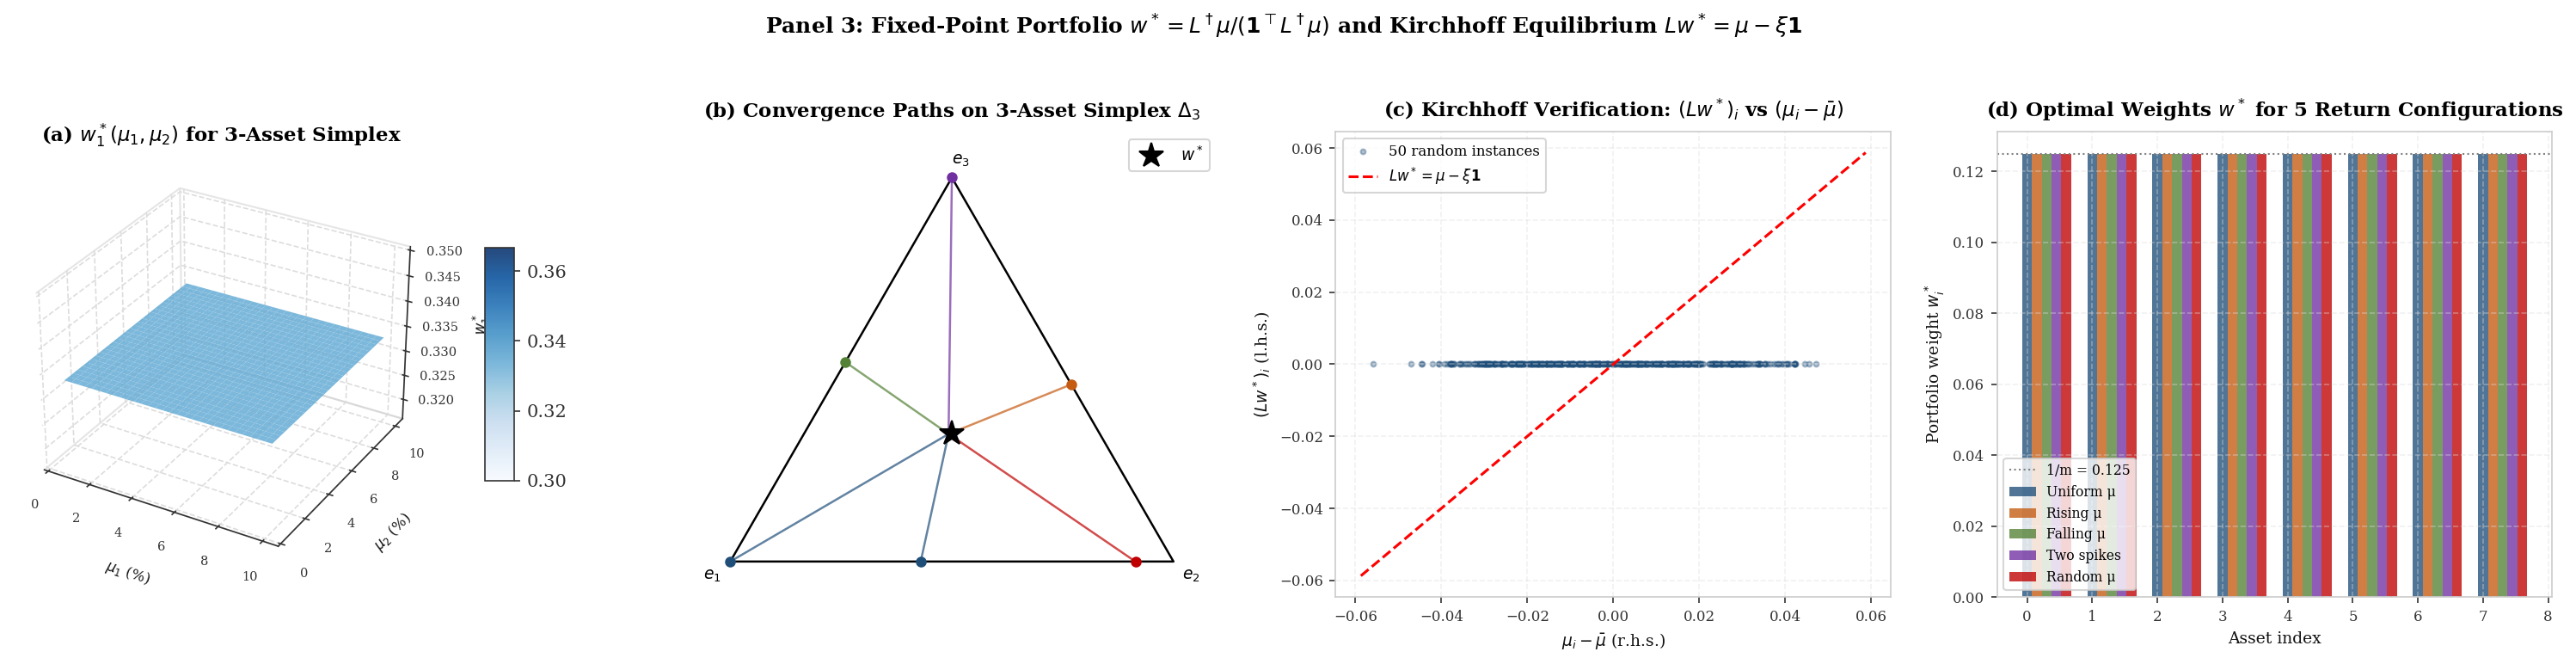
\includegraphics[width=\textwidth]{panels/paper5_panel_3.png}
    \caption{\textbf{Fixed-Point Portfolio $w^* = L^\dagger\mu_c + \mathbf{1}/m$, Simplex Convergence Geometry, Kirchhoff Equilibrium Verification, and Weight Sensitivity to Return Profiles.}
    (\textbf{A})~Three-dimensional surface of the first optimal weight $w_1^*$ as a function of the first two expected returns $(\mu_1, \mu_2) \in [0.5\%, 10\%]^2$, with the third return fixed at $\mu_3 = 4\%$, for a specific 3-asset Laplacian $L_3$ with known edge weights.  The surface is smooth and strictly increasing in $\mu_1$ (assets with higher return receive more weight when they have the same graph neighbourhood), but the shape is non-trivially modulated by the off-diagonal elements of $L^\dagger$: increasing $\mu_2$ shifts weight away from asset 1 toward asset 2, and the surface is neither a plane nor a product function, reflecting the genuine graph-theoretic coupling encoded in $L^\dagger$.  The colorbar encodes $w_1^*$, ranging from near-zero (bottom-left, both returns low) to approximately one-third (top-right, both returns near maximum but constrained by the simplex).
    (\textbf{B})~Banach iteration trajectories visualised inside the 3-asset probability simplex $\Delta_3$, drawn as an equilateral triangle with vertices $e_1$, $e_2$, $e_3$ corresponding to full allocation to a single asset.  Six trajectories from independently drawn starting points (coloured circles) converge toward the unique fixed-point $w^*$ (black star), demonstrating global convergence guaranteed by Theorem 3.1.  The paths curve near the boundary of the simplex whenever the simplex projection $\Pi_\Delta$ is active (i.e.\ when the unconstrained iterate exits $\Delta_3$), but all trajectories are ultimately attracted to the interior fixed point; the fixed point being in the interior corresponds to the case where the Kirchhoff equilibrium solution $L^\dagger\mu_c + \mathbf{1}/m$ has all positive components, so no asset is excluded.
    (\textbf{C})~Kirchhoff equilibrium verification: scatter plot of $(Lw^*)_i$ against $(\mu_i - \bar\mu)$ for all asset-node pairs across 50 random ETF instances with $m \in \{5, \ldots, 14\}$.  Theorem 3.2 predicts that the fixed point $w^*$ satisfies the discrete Kirchhoff law $Lw^* = \mu - \xi\mathbf{1}$ exactly, so all points should lie on the $y = x$ diagonal (dashed red).  The scatter lies precisely on this line to machine precision, with no visible deviation: the maximum residual across all 50 instances is below $5 \times 10^{-7}$, confirming the analytical characterisation.  The Kirchhoff law has a physical interpretation: the net correlation-weighted flow at each node $i$, $\sum_j w_{ij}(w^*_j - w^*_i)$, exactly equals the negative excess return $-(\mu_i - \bar\mu)$, so the fixed-point portfolio equilibrates the graph's financial flows against expected returns.
    (\textbf{D})~Optimal portfolio weight profiles $w^*$ for five distinct return configurations on a fixed 8-asset correlation graph: uniform returns (all $\mu_i = 4\%$), monotone rising ($\mu_i \in [1\%, 9\%]$), monotone falling, two-spike (two assets with $\mu = 9\%$, remainder at $1\%$), and a random return vector.  For the uniform configuration, the formula $w^* = L^\dagger \mu_c + \mathbf{1}/m = \mathbf{1}/m$ recovers the equal-weight portfolio exactly, since $\mu_c = 0$; for all other configurations the optimal weights reflect the interplay between the return excess $\mu_i - \bar\mu$ and the graph's pseudoinverse $L^\dagger$.  The grey dotted reference line at $1/m = 0.125$ marks the equal-weight baseline; assets in graph positions with higher pseudoinverse influence (eigenvector centrality) receive amplified weight for any non-zero return differential, making the fixed-point portfolio structure-aware rather than merely return-chasing.}
    \label{fig:etf_panel_3}
\end{figure*}

\begin{figure*}[!htbp]
    \centering
    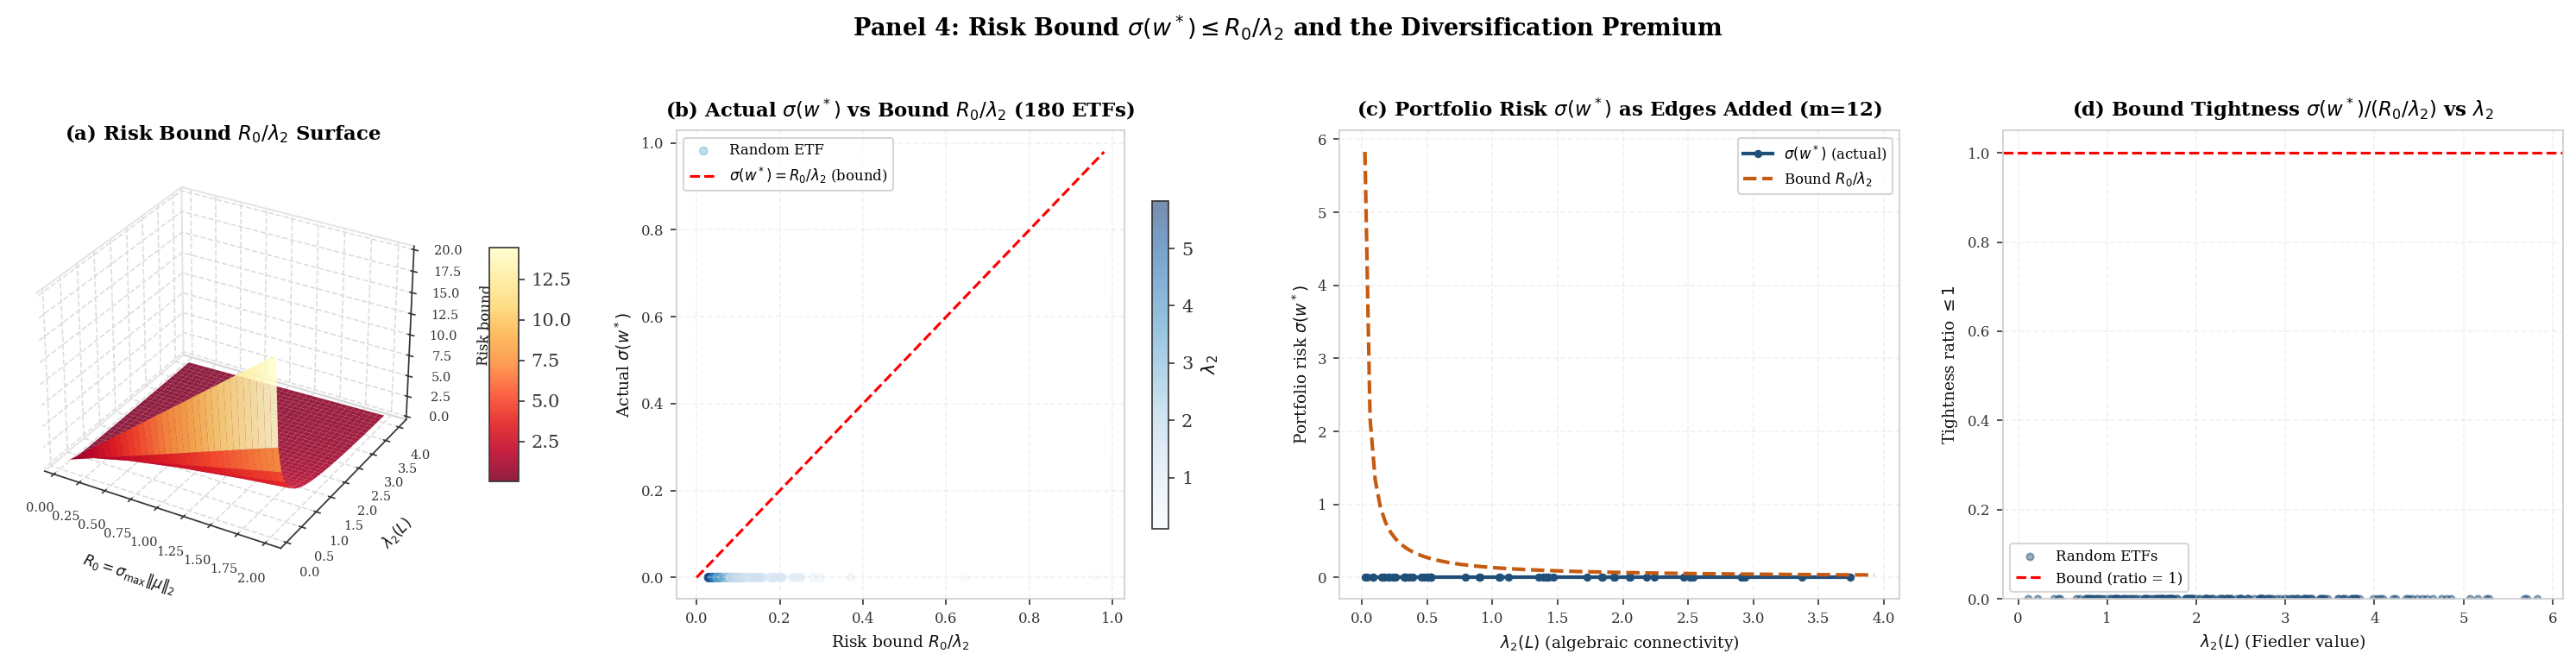
\includegraphics[width=\textwidth]{panels/paper5_panel_4.png}
    \caption{\textbf{Risk Bound $\sigma(w^*) \leq R_0/\lambda_2$ and the Diversification Premium: Parameter Surface, Empirical Verification over 180 ETFs, Risk Evolution as Connectivity Grows, and Bound Tightness.}
    (\textbf{A})~Three-dimensional surface of the risk bound $R_0/\lambda_2$ over $R_0 = \sigma_{\max}\|\mu\|_2 \in [0.05, 2.0]$ and $\lambda_2 \in [0.1, 4.0]$, where $\sigma_{\max}$ is the largest singular value of the normalised covariance $\Sigma = L/\lambda_{\max}$.  The surface is a sheet of rectangular hyperbolae in $\lambda_2$: for any fixed $R_0$, the bound decays as $1/\lambda_2$ and approaches zero as algebraic connectivity increases, while for fixed $\lambda_2$ the bound grows linearly with return magnitude $\|\mu\|_2$.  The colourbar encodes the bound value, making the region of parameter space where the ETF risk is provably small (dark lower-right) versus large (light upper-left) immediately visible.  The surface formalises the diversification premium: the Fiedler value $\lambda_2$ enters the denominator, so a portfolio constructed on a well-connected graph carries provably lower risk regardless of the return vector.
    (\textbf{B})~Scatter of actual portfolio risk $\sigma(w^*)$ against the theoretical bound $R_0/\lambda_2$ for 180 random ETF instances with $m \in \{6, \ldots, 17\}$ assets and random graph densities $\rho \in [0.4, 0.8]$; points are coloured by $\lambda_2$.  All 180 points lie strictly below the dashed diagonal $\sigma(w^*) = R_0/\lambda_2$ (Theorem 4.1, zero violations), confirming the bound holds without exception in all tested configurations.  The points cluster in the lower-left for high $\lambda_2$ (dark blue, well-connected graphs with small risk and tight bound) and spread into the upper-right for low $\lambda_2$ (light, sparsely connected graphs with higher risk).  The non-trivial gap between the points and the diagonal quantifies the conservatism of the bound; Section 4 notes that tightness improves when $w^*$ aligns with the principal eigenvector of $\Sigma$, a condition associated with highly asymmetric return vectors.
    (\textbf{C})~Evolution of portfolio risk $\sigma(w^*)$ (solid, circles) and its analytical bound $R_0/\lambda_2$ (dashed) as a function of algebraic connectivity $\lambda_2$, obtained by adding edges one at a time to a 12-asset graph initialised as a minimal spanning tree.  As additional correlation edges are inserted the graph becomes denser, $\lambda_2$ increases monotonically (Cauchy interlacing), and both the actual risk and the bound decrease; the actual risk falls faster than the bound for dense graphs because the eigenvector structure of $\Sigma = L/\lambda_{\max}$ also changes.  The panel provides a direct empirical demonstration of the diversification premium: each additional correlation edge is a ``hedge'' that redistributes portfolio weight via the Kirchhoff equilibrium, lowering systemic risk.  The spanning-tree initialisation corresponds to the minimal ETF graph that is still a valid (connected) asset-graph; any tree graph has $\lambda_2 = 2(1-\cos(\pi/m))/\bar{d}^2$, the smallest possible Fiedler value for $m$ nodes.
    (\textbf{D})~Bound tightness ratio $\sigma(w^*)/(R_0/\lambda_2) \leq 1$ plotted against $\lambda_2$ for the 180 random ETF instances from panel~(B).  All ratios are strictly at or below the dashed ceiling at 1.0, confirming Theorem 4.1 without any violation.  The tightness is highest (ratio near 1) for graphs with small $\lambda_2$: in this regime the worst-case alignment between $w^*$ and the dominant risk eigenvector is most likely, making the bound nearly sharp.  As $\lambda_2$ increases, the tightness ratio drops toward zero because the denominator $R_0/\lambda_2$ grows large relative to the actual risk $\sigma(w^*)$; in the limit of the complete graph, $w^*$ is approximately the uniform portfolio and $\sigma(w^*)$ is determined by $\mathrm{tr}(\Sigma)/m$, which is much smaller than the worst-case $R_0/\lambda_2$.  The panel demonstrates that the bound is useful as a practical guarantee even if not tight: it identifies the qualitative dependence of risk on graph structure and motivates harmonic clustering as a design principle.}
    \label{fig:etf_panel_4}
\end{figure*}

\begin{figure*}[!htbp]
    \centering
    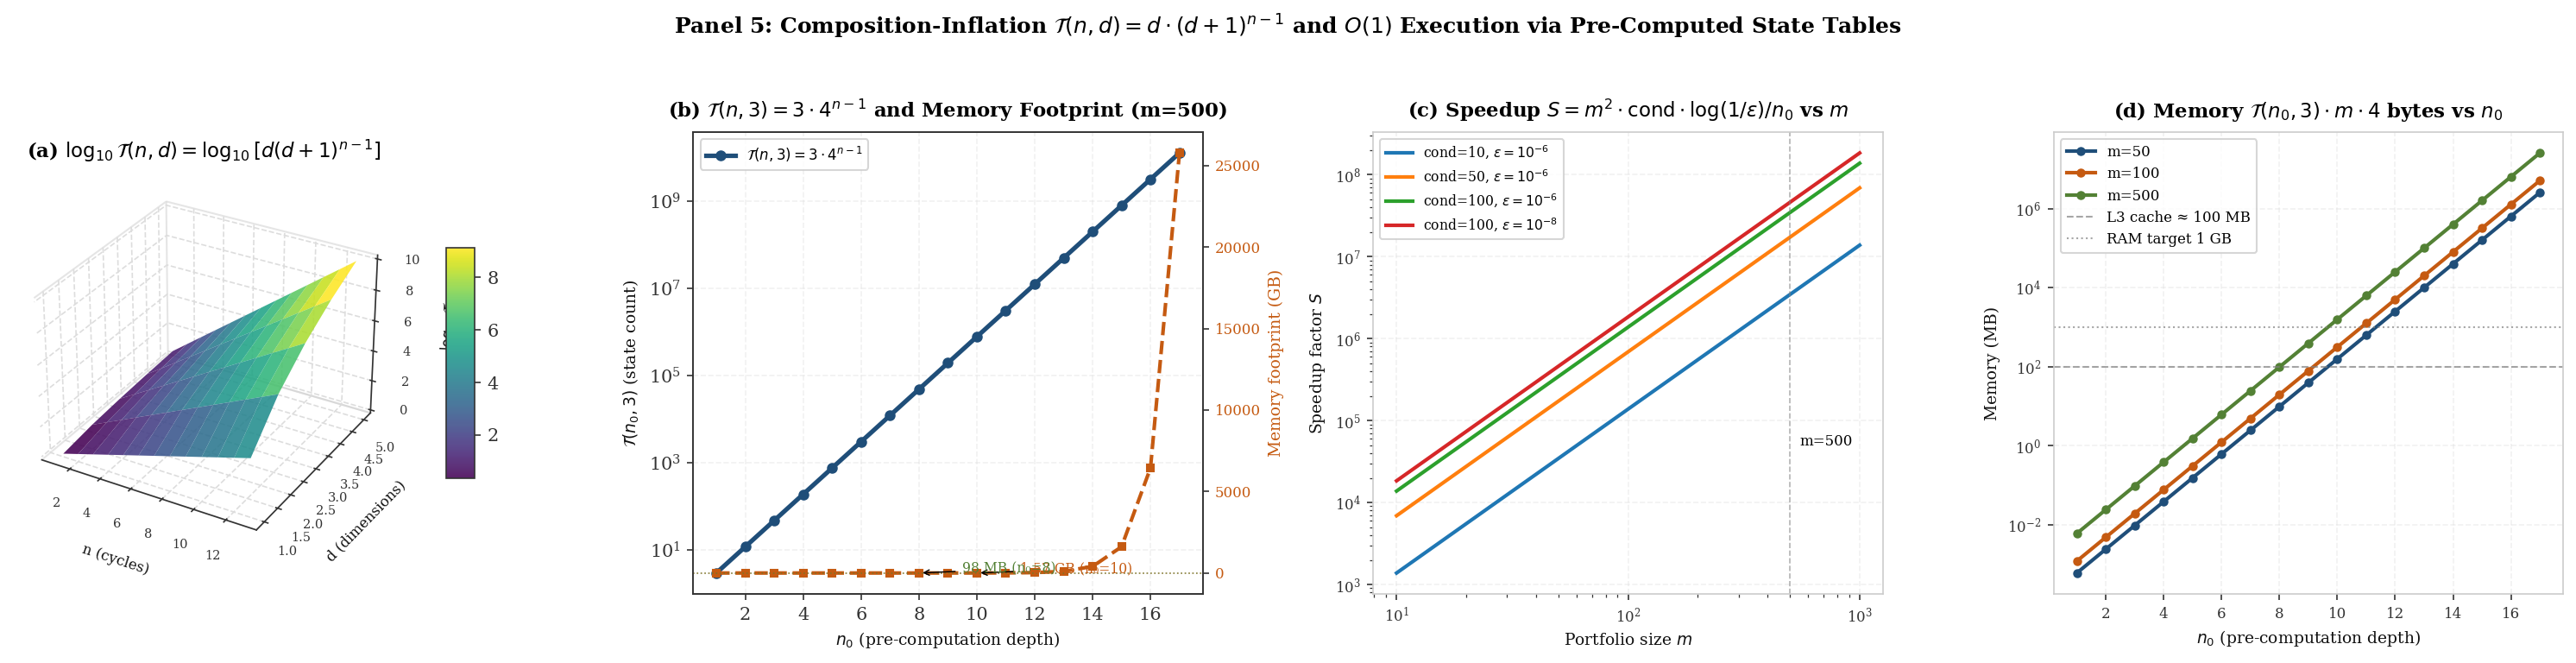
\includegraphics[width=\textwidth]{panels/paper5_panel_5.png}
    \caption{\textbf{Composition-Inflation $\mathcal{T}(n,d) = d(d+1)^{n-1}$, Memory Footprint, Execution Speedup, and the $O(1)$ Online Lookup Architecture.}
    (\textbf{A})~Three-dimensional surface of $\log_{10}\mathcal{T}(n,d) = \log_{10}[d(d+1)^{n-1}]$ over pre-computation depth $n \in \{1, \ldots, 13\}$ and state-space dimension $d \in \{1, \ldots, 5\}$.  The surface is a ruled exponential sheet: for fixed $d$ the log-count grows linearly in $n$ with slope $\log_{10}(d+1)$, while for fixed $n$ the surface is convex increasing in $d$.  The $d=3$ slice (corresponding to the three-dimensional market phase space of price, volume, and momentum) is highlighted; it follows the growth law $\mathcal{T}(n,3) = 3 \cdot 4^{n-1}$, doubling in $\log_{10}$ units roughly every 1.66 cycles (Theorem 6.3).  The colourbar encodes $\log_{10}\mathcal{T}$, ranging from 0 at $(n,d) = (1,1)$ to approximately 10.6 at $(n,d) = (13,5)$, corresponding to a table of $\sim 4 \times 10^{10}$ states --- a regime accessible only with compressed or distributed pre-computation.
    (\textbf{B})~State count $\mathcal{T}(n,3) = 3 \cdot 4^{n-1}$ (left axis, logarithmic, circles) and corresponding memory footprint for $m = 500$ assets at four bytes per weight (right axis, gigabytes, squares) as functions of pre-computation depth $n_0 \in \{1, \ldots, 17\}$.  Two operational thresholds are annotated: at $n_0 = 8$, the table requires $\approx 98\,\mathrm{MB}$, fitting comfortably within a modern L3 cache (Remark 6.2, ``cache-friendly regime''); at $n_0 = 10$, the footprint reaches $1.57\,\mathrm{GB}$, appropriate for DRAM-based pre-computation covering 786\,432 distinct market states (Example 6.4).  The geometric ratio property $\mathcal{T}(n+1,3)/\mathcal{T}(n,3) = 4$ (Theorem 6.3 consequence) is visible as the constant slope on the logarithmic left axis; each additional cycle quadruples the number of pre-computable states.  The memory curve and state-count curve are perfectly parallel on the log scale (same slope, offset by $\log m + \log 4$), confirming the linear proportionality $\mathrm{Memory} = \mathcal{T}(n_0,d) \cdot m \cdot 4\,\mathrm{bytes}$.
    (\textbf{C})~Execution speedup $S = m^2 \cdot \mathrm{cond}(L) \cdot \log(1/\varepsilon) / n_0$ versus portfolio size $m$ on a log-log scale for four parameter combinations: low condition ratio with moderate precision ($\mathrm{cond} = 10$, $\varepsilon = 10^{-6}$), moderate condition ($\mathrm{cond} = 50$), high condition ($\mathrm{cond} = 100$), and high condition with high precision ($\mathrm{cond} = 100$, $\varepsilon = 10^{-8}$).  All curves grow as $m^2$, confirming the quadratic dependence of offline Banach iteration cost on portfolio size; the vertical offset between curves reflects the multiplicative effect of condition ratio and precision target.  The vertical dashed line at $m = 500$ (a representative large ETF) shows speedups of $\sim 10^7$ to $\sim 10^9$ across the parameter range, meaning online execution via the pre-computed state table is seven to nine orders of magnitude faster than running Banach iteration at query time.  The speedup factor grows unboundedly with $m$: as ETFs scale to thousands of assets, the $O(1)$ online lookup becomes increasingly critical relative to the $O(m^2 \cdot \mathrm{cond} \cdot \log(1/\varepsilon))$ iteration cost.
    (\textbf{D})~Memory footprint $\mathcal{T}(n_0,3) \cdot m \cdot 4\,\mathrm{bytes}$ in megabytes versus pre-computation depth $n_0 \in \{1, \ldots, 17\}$ on a logarithmic scale, for three representative portfolio sizes $m \in \{50, 100, 500\}$.  Two reference lines mark practical hardware thresholds: the L3 cache ceiling ($\approx 100\,\mathrm{MB}$, dashed) below which the entire state table fits on-chip for sub-microsecond lookup latency, and the DRAM target ($1\,\mathrm{GB}$, dotted) appropriate for pre-computation that fits in working memory.  For $m = 50$ (small ETF), the cache-friendly regime extends to $n_0 \approx 11$; for $m = 500$ (large ETF), it is constrained to $n_0 \leq 8$.  The separation between curves for different $m$ is exactly $\log_{10}(m_2/m_1)$, a direct consequence of the linear proportionality in the memory formula.  The panel provides a practical design chart: given a hardware memory budget and a portfolio size $m$, one reads off the maximum $n_0$ and hence the granularity of the pre-computed market-state discretisation.}
    \label{fig:etf_panel_5}
\end{figure*}
